\chapter{Weight Reparametrization}

\begin{abstract}
    abstract of this part
\end{abstract}

\section{Introduction And Related Work}
% region
The introduction of neural networks has revolutionised the field of machine
learning, leading to breakthroughs in various areas such as image and speech
recognition, natural language processing, and game playing. However, the size of
neural networks has steadily increased in recent years, largely thanks to the
availability of powerful \ac{GPUs}. They have made it possible to train larger
and more complex models. However, as the size of neural networks has grown, so
have the computational and memory requirements to train and deploy them. The
evolution of neural network architectures can be traced back to the Rosenblatt
Perceptron \cite{rosenblatt1958perceptron}, a single-layer feedforward network
with only one neuron. Over time, neural network architectures became more
complex and began to include multiple layers, known as multilayer perceptron, or
fully connected networks. Then, with the introduction of \ac{CNNs}, neural
network architectures for image recognition have grown even larger.
Convolutional neural networks use convolutional layers to automatically and
adaptively learn spatial hierarchies of features from input images. This allows
\ac{CNNs} to effectively learn and classify images with high accuracy. Some of
the most notable \ac{CNN} architectures include AlexNet
\cite{DBLP:conf/nips/KrizhevskySH12}, which was developed in 2012 and has 60
million parameters. The VGG networks \cite{DBLP:journals/corr/SimonyanZ14a},
developed in 2014, are ranging from 132 to 143 million parameters. Inception
\cite{DBLP:conf/cvpr/SzegedyLJSRAEVR15}, developed in 2014, had 27 million
parameters in its third version. And the ResNet networks
\cite{DBLP:conf/cvpr/HeZRS16}, developed in 2015, are ranging from 11 to 60
million parameters. \\


The need for neural networks in embedded applications has grown in recent years,
with examples such as object detection in self-driving cars, image and speech
recognition in mobile devices, and natural language processing in smart
speakers. These applications require real-time processing and low power
consumption, which are impossible with large neural networks. Pruning techniques
can reduce the size of neural networks, making them more suitable for deployment
on embedded devices while still maintaining or even improving their performance.
Methods such as structured and unstructured weight pruning can reduce the number
of parameters and FLOPS, consequently reducing the network's size, memory and
power consumption.\\


Pruning is an excellent way to obtain lightweight neural networks because it
reduces the number of parameters in a pre-trained network without the need to
design a new architecture from the ground up. Instead of starting from scratch,
pruning techniques can be applied to existing architectures, which have been
trained and tested on large-scale datasets. It aims at reducing the number of
parameters in a network by removing redundant or unnecessary weights. Pruning
methods can be split into two major categories: unstructured weight pruning,
where individual weights of the network are removed based on their importance.
And structured pruning, where entire columns, rows, channels, filters or even
subnetworks are removed. \\


The first methods to prune shallow networks were proposed in the late 1980s.
Techniques from that area include removing the smallest connection
\cite{janowsky1989pruning}, introducing a weight scaling factor and the study of
its impact on the loss function \cite{DBLP:conf/nips/MozerS88} or the study of
the sensitivity of the weights based on the gradients
\cite{DBLP:journals/tnn/Karnin90}. Most influential papers of the early pruning
days are Optimal Brain Damage \cite{DBLP:conf/nips/CunDS89} and Optimal Brain
Surgeon
\cite{DBLP:conf/nips/HassibiS92,DBLP:conf/nips/HassibiSW93,DBLP:conf/icnn/HassibiSW93}.
The former work focuses on pruning weights based on their impact on the loss,
approximated by its Taylor series, which requires the computation of the hessian
matrix of the loss. However, computing the hessian matrix is Intractable in
practice due to the large number of parameters in the neural networks.
Therefore, the authors introduced a few simplifying assumptions, most notably
the diagonal assumption for the hessian matrix: loss perturbations following
weight pruning are assumed to be weight independent. \\


More recently, pruning regained traction with the work of Han et al.
\cite{DBLP:conf/nips/HanPTD15}.  The authors introduced a three-step pruning
method where first, the weights are tuned. Then all the weights whose absolute
value is below a certain threshold are removed. Finally, the remaining weights
are finetuned. \\


Following this work, research efforts stirred toward structured pruning.
Structured pruning removes groups of weights. The substructure of this group can
be a simple row or column in a filter, a channel of a filter, the filter itself
or even entire subnetworks. Structured pruning is not sparsifying weight
tensors, but rather reshaping the network to remove unnecessary parts of it that
are costly to evaluate and do not bring much performance improvement regarding
the considered task. Since the remaining weight tensors are not sparse, speedups
can be achieved with conventional libraries and hardware. In this context, Anwar
et al. \cite{anwar2017structured} proposed a pruning technique on various levels
(channels, kernels and intra-kernel levels) while Li et al.
\cite{DBLP:conf/iclr/0022KDSG17} proposed a pruning method at a larger (filter)
level. Network slimming \cite{DBLP:conf/iccv/LiuLSHYZ17} is a streamlined
approach that aims at pruning the most useless channels in the layers preceding
\ac{batch norm} \cite{DBLP:conf/icml/IoffeS15}. It induces sparsity with
$\ell_1$ penalization of the \ac{batch norm} scaling factors, each one
associated with a channel. Then channels are removed based on the relative
importance of their associated scaling factor, up to a predefined sparsity
ratio. More recent work proposed an automatic policy for pruning, such as
\ac{amc} \cite{DBLP:conf/eccv/HeLLWLH18} which relies on reinforcement learning
with two interacting agents; the first one iterates over the layers of the
architecture and defines a targeted sparsity, and the second agent implements
the targeted sparsity using channel pruning. The \ac{amc} algorithm is either
constrained by accuracy or efficiency, depending on the reward assigned to the
agents.  Going further with the concept of automatic pruning and architecture
search, Ramakrishnan et al. \cite{DBLP:conf/crv/RamakrishnanSN20} adapt $\ell_1$
penalization from \cite{DBLP:conf/iccv/LiuLSHYZ17} to model the relative
importance of layers, groups of layers or network parts that can be removed.
Following the same line, \cite{DBLP:conf/icml/KangH20} proposed a channel
pruning method based on batch normalization parameters. The authors introduce
masks which model the likelihood of feature maps being inhibited by the ReLU
activation function and thereby not contributing to the evaluation of the
underlying network. These masks are obtained by binarizing the cumulative
density function of the gaussian distribution parameterised by the scaling and
the shift of the BN layer. Masks and BN parameters are updated “end-to-end” with
a gradient estimated using the Gumble Softmax trick
\cite{DBLP:conf/iclr/JangGP17}. Authors claim that a high accuracy is maintained
after pruning and without fine-tuning. \\



Although convenient to implement in practice, structured pruning imposes a
strong topological prior by removing whole chunks in the primary network and
achieves a lower sparsity rate compared to unstructured pruning. On the other
hand, unstructured weight pruning focuses on removing independent weights from
the global structure. As a result, this method is much more flexible and leads
to high sparsity rates and compression ratios. Han et al.
\cite{DBLP:conf/nips/HanPTD15} introduced a simple yet effective three-step
algorithm for unstructured weight pruning: a first standard training step to
identify the most important connections, a magnitude pruning step to remove the
smallest weight and a final finetuning step to compensate for the loss of
accuracy. \cite{DBLP:journals/corr/HanMD15} used the same technique in
combination with quantization and Huffman coding, achieving a compression ratio
of up to 49x for a VGG16 network. Other methods do not rely on weight magnitude
such as \cite{DBLP:conf/iclr/LouizosWK18}, which uses non-negative stochastic
gates as a surrogate L0 norm and penalise non-zero weights during training.
Variational Dropout \cite{DBLP:conf/icml/MolchanovAV17} introduces a
multiplicative gaussian noise as an alternative to binary dropout
\cite{DBLP:journals/corr/abs-1207-0580,DBLP:journals/jmlr/SrivastavaHKSS14} with
an unbound dropout rate. Magnitude pruning regains significant attention after
the publication of the Lottery Ticket Hypothesis
\cite{DBLP:conf/iclr/FrankleC19}ttery Tickets, whose training with initial
weights taken from the large networks yields comparably accurate classifiers. To
extract the lottery ticket, it is necessary to train the large network up to
convergence, apply magnitude pruning and restore the original values of the
unpruned weights. This Lottery Ticket can then be trained to match the level of
performances of the large network, with at most the same number of epochs
needed. Although remarkable, this result is hardly applicable in practice since
it requires multiple computationally intensive training steps.\\


These structured or unstructured methods propose different saliency indicators
and pruning criteria that aim at identifying and removing redundant or
unnecessary weights or groups of weights in order to remove them. Removing
weights introduces a loss of functional performance - depending on the task
considered - that needs to be compensated for (with the exception of
\cite{DBLP:conf/icml/KangH20}). This is achieved through finetuning the sparse
or lightened networks obtained after applying the pruning criterion. Finetuning
is a computationally intensive task and requires additional training time.
Moreover, the amount of weights pruned is enforced after the initial training,
meaning that the final target size or weight budget is never considered in the
optimization procedure. Hence the need for a finetuning step. \\


In order to address the aforementioned issues, we introduce a novel
reparametrization that learns not only the weights of a surrogate lightweight
network but also its topology. This reparametrization acts as a regulariser that
models the tensor of the parameters of the surrogate network as the Hadamard
product of a weight tensor and an implicit mask. The latter makes it possible to
implement unstructured pruning constrained with a budget loss that precisely
controls the number of nonzero connections in the resulting network. Experiments
conducted on the CIFAR10 and the TinyImageNet classification tasks, using
standard primary architectures (namely Conv4, VGG19 and ResNet18), show the
ability of our method to train effective surrogate pruned networks without any
fine-tuning.

% endregion

\section{Pruning With Weight Reparametrization And Budget Loss}
% region
Consider the general case of a multi-layer neural network, denoted as a function
$f$ of two variables: $\theta$ and $X$. $f$ can be seen as the topology of the
network: a computation graph whose edge values are given by $\theta$. Indeed,
$\theta$ is the set of weights of the network: $\theta = \{\mathbf{w}_1,
\mathbf{w}_2, \ldots, \mathbf{w}_L\}$, where $L$ is the number of layer of the
network. $X$ is the input taken by the network. The input $X$ is an element of a
dataset $\mathcal{D}=\{ \mathcal{X}, \mathcal{Y} \}$, where $\mathcal{X}$ is the
set of the input data, and $\mathcal{Y}$ is the set of the corresponding labels.
The elements of $\mathcal{X}$ and $\mathcal{Y}$ are real-valued tensors.

\begin{equation}
    % \centering
    \begingroup
  \setlength\arraycolsep{0pt}
  f \colon\begin{array}[t]{c >{{}}c<{{}} c}
             \mathbb{R}^{\dim (X)} & \to & \mathbb{R}^{\dim (y)} \\ 
             X & \mapsto & f(X, \theta) = \hat{y} 
          \end{array}
  \endgroup
\end{equation}

Evaluating the neural network $f(X_i, \theta)$ yields the output $\hat{y_i}$
which is the prediction of the network for the input $X_i$. The discrepancy
between the output of the neural network $\hat{y_i}$ and the ground truth $y_i
\in \mathcal{Y}$ is computed with a loss function $\mathcal{L}$.  This loss is
then minimized by updating the parameters $\theta$ of the network, thanks to the
backpropagation \cite{rumelhart1985learning,rumelhart1986learning} and gradient
descent methods.\\

The $L_0$ norm is perfectly suited for introducing sparsity in a network by, on
the one hand, acting as a sparsity-inducing regulariser for the weights, and on
the other hand, by indicating the number of non-zero weights in the network,
which is useful for computing the weight budget. \\

Our aim is to propose an end-to-end method that fits into the backpropagation
framework. Therefore, adding a $L_0$ regulariser and a $L_0$ based weight budget
is not possible since $L_0$ norm is not differentiable. Thus we propose our
differentiable reparametrization, which seeks to define a novel weight
expression related to magnitude pruning
\cite{DBLP:conf/nips/CunDS89,DBLP:conf/nips/HanPTD15}. This expression
corresponds to the Hadamard product involving a weight tensor and a function
applied entry-wise to the same tensor (as shown in
\cref{fig:chap1:comparison_reparam_vs_mag_pruning}). This function acts as a
mask that i) multiplies weights by soft-pruning factors which capture their
importance and ii) pushes less important weights to zero through a particular
budget added to the loss function $\mathcal{L}$. \\

\begin{figure}[h]
    \centerline{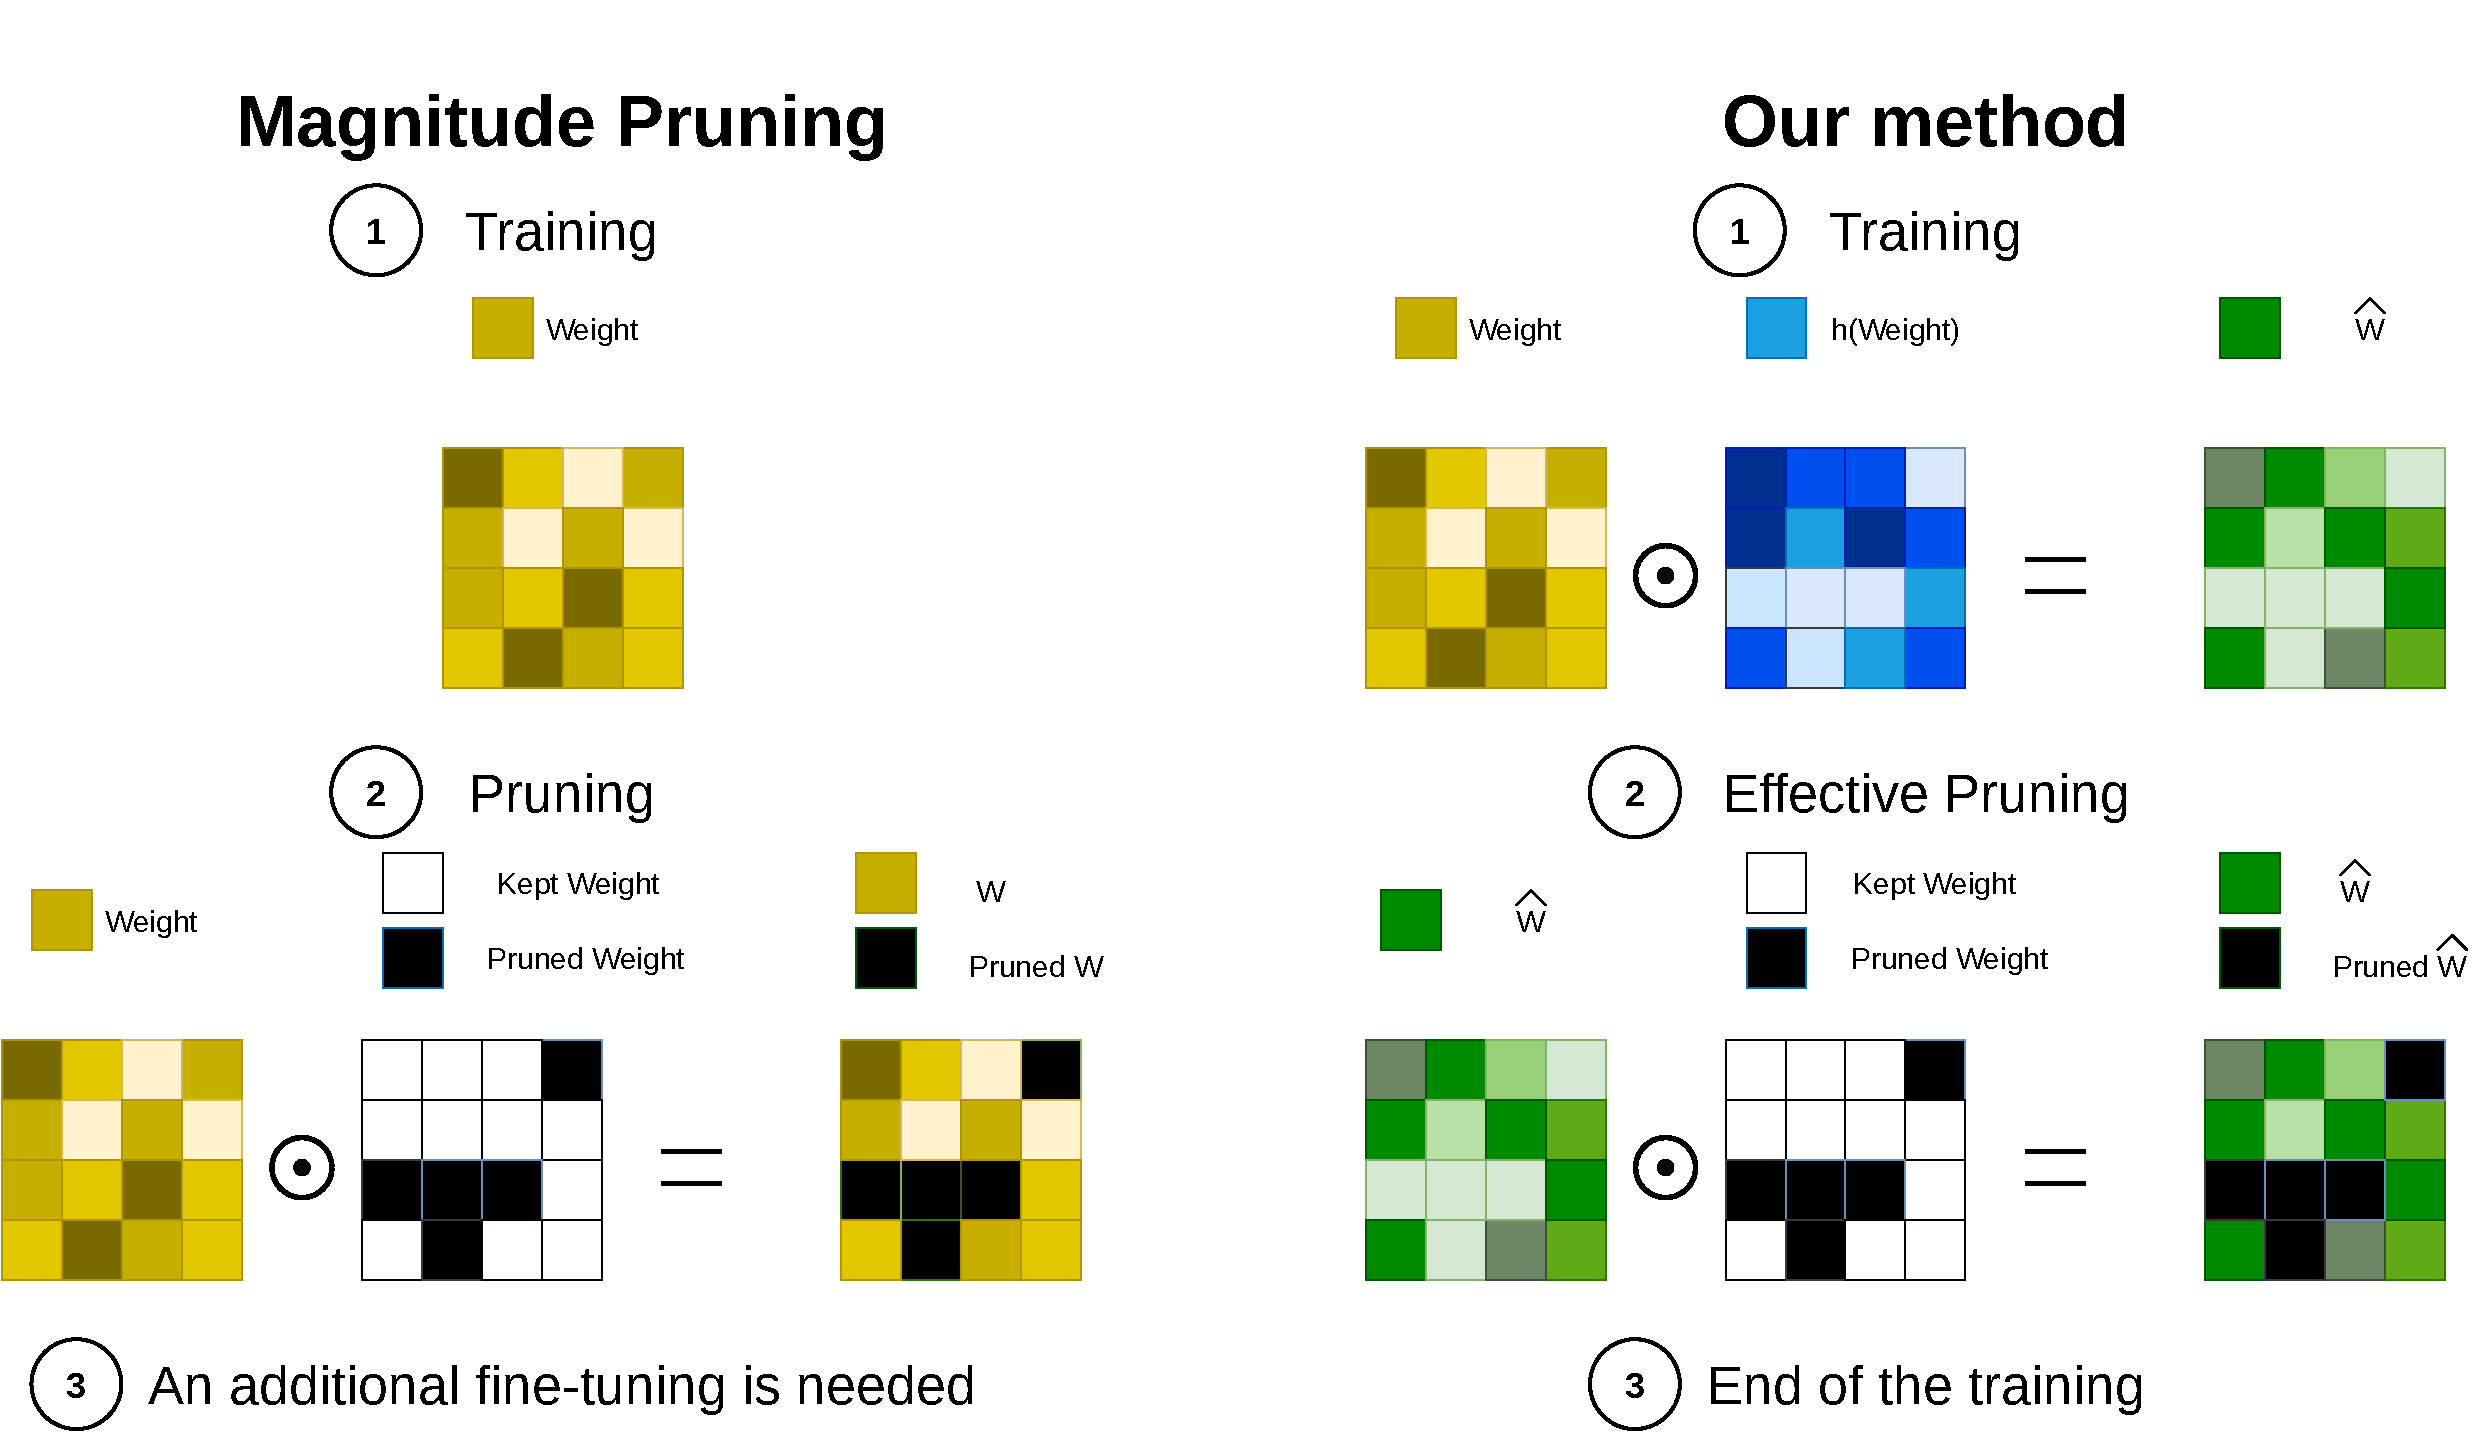
\includegraphics[width=12.5cm]{chapter_1/assets/comparison_reparam_vs_mag_pruning.pdf}}
  \caption{Comparison of our method and magnitude pruning. Magnitude pruning
  does not include any prior on weights during the initial training phase
  and needs an additional fine-tuning procedure. Our method embeds a saliency
  heuristic based on the weight magnitude in the weight reparametrization and
  does not require fine-tuning.}
  \label{fig:chap1:comparison_reparam_vs_mag_pruning}
\end{figure}


Our proposed framework allows for a joint optimization of the network weights
and topology. On the one hand, it prevents disconnections which may lead to
degenerate networks with an irrecoverable performance drop. On the other hand,
it allows reaching a targeted pruning budget in a more convenient way than $L_1$
regularization. Our reparametrization also helps minimize the discrepancy
between the primary and the surrogate networks by maintaining competitive
performances without fine-tuning. Learning the surrogate network requires only
one step that achieves pruning as a part of network design. This step zeroes out
the targeted number of connections by constraining their reparametrized weights
to vanish.

\subsection{Weight Reparametrization}
\label{sec:chap1:weight_reparam}

We consider the primary network $f$ as a combination of $L$ layers. The global
expression of $f$ can be recursively defined by the application of the layer $\ell$
to the output of the layer $\ell-1$. Without a loss of generality, we omit the
bias for the sake of clarity. This expression is shown on
\cref{eqn:chap1:layer_eq_f}.
\begin{equation}
\label{eqn:chap1:layer_eq_f}
f(\mathbf{x}) = g_L \big(\mathbf{w}_L \cdot g_{L-1}(\mathbf{w}_{L-1} \cdot g_{L-2} \dots
\mathbf{w}_2 \cdot g_1(\mathbf{w}_1 \cdot \mathbf{x}))\big),
\end{equation}
\noindent with $g_\ell$ being a nonlinear activation associated to $\ell \in
\left\{ 1,\dots, L \right\}$ and $\left\{ \mathbf{w}_\ell \right\}_\ell$ a
weight tensor. Keeping the same topology but changing the values of the weight,
we now consider the surrogate network $\hat{f}$ with weights
$\{\hat{w}_\ell\}_\ell$. \Cref{eqn:chap1:layer_eq_f} now becomes
\cref{eqn:chap1:layer_eq_f_hat}. The activation function and the topology of $f$
and $\hat{f}$ are the same. Only the weights are changing.

\begin{equation}
\label{eqn:chap1:layer_eq_f_hat}
\hat{f}(\mathbf{x}) = g_L \big(\mathbf{\hat w}_L \cdot g_{L-1}(\mathbf{\hat w}_{L-1} \cdot g_{L-2}
\dots\mathbf{\hat w}_2 \cdot g_1(\mathbf{\hat w}_1 \cdot \mathbf{x}))\big).
\end{equation}

\noindent In the above \cref{eqn:chap1:layer_eq_f_hat}, $\mathbf{\hat w}_\ell$
is referred to as apparent weight. The apparent weight is a reparametrization of
$\mathbf{w}_\ell$, that includes a prior on its saliency. An apparent weight
$\mathbf{\hat w}_\ell$ of $\hat{f}$ is derived from the standard weight
$\mathbf{w}_\ell$ of $f$ by applying the following reparametrization: 
\begin{equation}
  \label{eqn:reparam}
  \mathbf{\hat w}_\ell = \mathbf{w}_\ell  \odot h_t(\mathbf{w}_\ell),
\end{equation}
\noindent with $h_t$ being the reparametrization function and $t$ its
temperature parameter. Here, $\odot$ represents the Hadamar product. It means
that the reparametrization is element-wise, and every single weight has its own
reparametrization. This reparametrization function enforces the prior that
smallest weights should be removed from the network and act as a surrogate $L_0$
norm for the budget loss (see \cref{sec:chap1:budget_loss}). In order to achieve
this objective, $h_t$ should exhibit four properties: \\

\begin{enumerate}
  \item $\forall x \in \mathds{R},~~ 0 \leq h_t(x) \leq 1 $
  \item $h_t(x) \in C^1 \text{ on } \mathds{R}$
  \item $h_t(x) = h_t(-x)$
  \item $\forall a,\varepsilon \in\mathds{R}^{+\ast},~ \exists ~t
  \in\mathds{R}^{+\ast} ~ | ~ h_t(x) \leq \varepsilon, x \in [-a,a]$
\end{enumerate}

\noindent\textbf{First Property - Constrained Image} \\
\begin{equation}
    \centering
    \forall x \in \mathds{R},~~ 0 \leq h_t(x) \leq 1
    \label{eqn:chap1:reparam_prop1}
\end{equation}
\\
There should not be any co-adaptation between the weights and their
reparametrization. Indeed, the reparametrization function should not act as a
scaling factor for the weight and scale it so that the apparent weight is larger
than the original weight. Finally, the apparent weight should have the same sign
as the original weight. That's why the image of $\mathbb{R}$ by $h_t$ should be
the segment $[0,1]$.\\

\noindent\textbf{Second Property - Differentiability} \\
\begin{equation}
    \centering
    h_t(x) \in C^1 \text{ on } \mathds{R}
    \label{eqn:chap1:reparam_prop2}
\end{equation}
\\
Our method should fit in the backpropagation method. Since the optimization will
be achieved by gradient descent, the reparametrization function should be
derivable to ensure that it has a computable gradient.\\

\noindent\textbf{Third Property - Symmetry} \\

\begin{equation}
    \centering
    h_t(x) = h_t(-x)
    \label{eqn:chap1:reparam_prop3}
\end{equation}
\\
The reparametrization function should not induce any bias toward the positive or
negative weights so that only their magnitudes matter. It implies that the
reparametrization function should be symmetric with respect to the origin.\\


\noindent\textbf{Fourth Property - Upper Bounded Segment} \\

\begin{equation}
    \centering
    \forall a,\varepsilon \in\mathds{R}^{+\ast},~ \exists ~t
    \in\mathds{R}^{+\ast} ~ | ~ h_t(x) \leq \varepsilon, x \in [-a,a]
    \label{eqn:chap1:reparam_prop4}
\end{equation}
\\
The last property ensures the existence of a temperature parameter $t$, which
allows upper-bounding the response of $h_t$ on any interval for any arbitrary
$\varepsilon$. More formally, for any arbitrarily large $a$ and arbitrarily
small $\varepsilon$, it exists a temperature $t$ which guarantees that the
reparametrization of any $x$ is smaller than $\varepsilon$, provided that $x$ is
in the segment $[-a, a]$. Hence, $h_t$ acts as a stopband filter which
eliminates the smallest weights where the parameter $t$ controls the width of
that filter. \\



\begin{figure}
    \centering
    \subfloat[$h_{t}$ with $t=1$ and varying $n$]{
        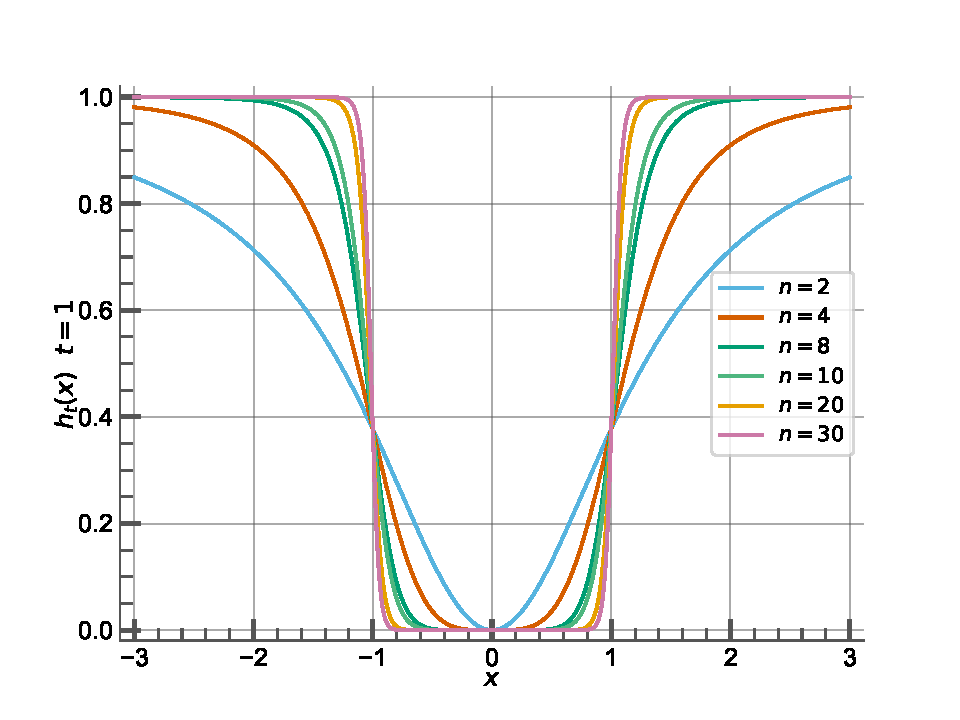
\includegraphics[width=0.49\linewidth]{chapter_1/assets/reparam_funct_varying_n.pdf}
        \label{fig:chap1:reparam_funct_varying_n}} \subfloat[$h_{t}$ with $n=2$
    and varying $t$]{
        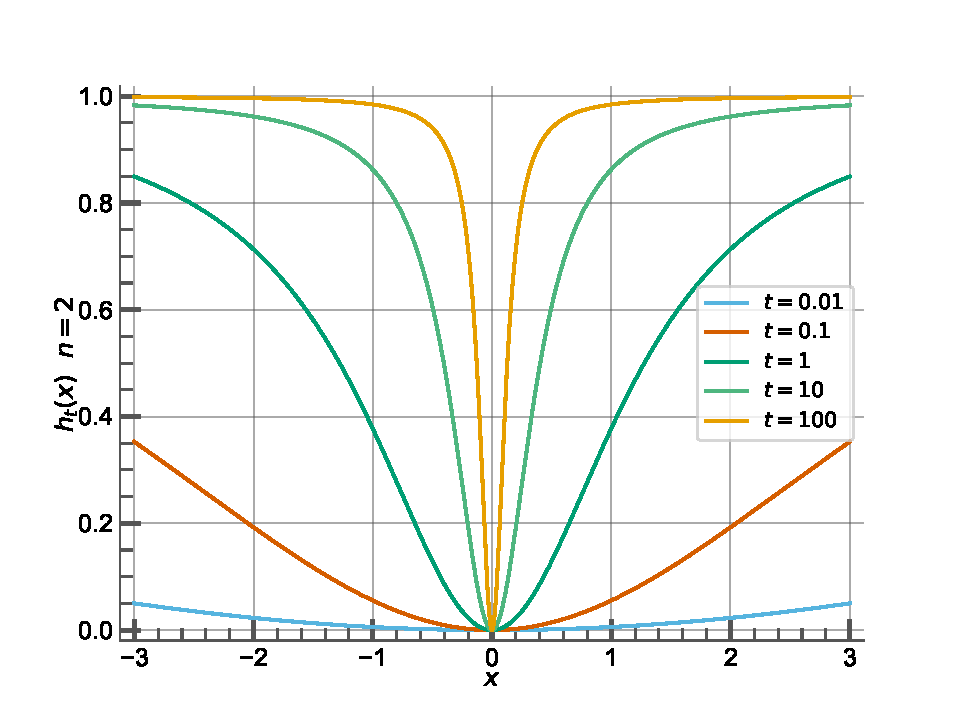
\includegraphics[width=0.49\linewidth]{chapter_1/assets/reparam_funct_varying_t.pdf}
        \label{fig:chap1:reparam_funct_varying_t}} \caption{\centering
    Reparametrization function $h_t$ with varying temperature parameter $t$ and
    power $n$. $t$ controls the width of the pit and $n$ controls the steepness
    of the slope.}
    \label{fig:stopband}
\end{figure}

Weight distribution varies greatly from one layer to another. In order to match
a specific budget (see \cref{sec:chap1:budget_loss}), the width of the stopband,
controlled by $t$, is tuned according to the weight distribution of each layer.
The manual setting of this parameter is difficult and cumbersome, so in
practice, $t$ is learned as a part of gradient descent on a layer-by-layer
basis.\\

% TODO: Ajouter amorce pour discussions sur l'initialisation de la température.
%the initial setting  $t_\text{init}$ of this temperature is shown in
%\cref{tbl:pruningperformances}.\\


Considering the aforementioned four properties of $h_t$, a simple choice of that
function is 
\begin{equation}
  \label{eqn:chap1:h_star_expression}
  h_t^*(x) = \exp\bigg\{{-\displaystyle\frac{1}{(tx)^n}}\bigg\}, ~ n\in 2\mathds{N},
\end{equation}
\noindent where $n$ controls the crispness of $h_t^*$. $n$ is not considered as
a parameter of $h_t$ (or $h_t^*$) since we use a fixed value for our
experiements, whereas $t$ is a learnt parameter and varies from one layer to
another. Although the function described in \cref{eqn:chap1:h_star_expression}
satisfies the four above properties, $h_t^*$ suffers from numerical instability
as it generates \ac{nan} outputs in most of the widely used deep learning
frameworks. Due to the way Backpropagation works, a single \ac{nan} in a weight
tensor makes the whole optimization process for the entire network no longer
possible. We consider instead a stabilized variant with a similar behavior, as
\cref{eqn:chap1:h_star_expression},  that still satisfies the four above
properties (see also \cref{fig:chap1:h_stable_vs_unstable}). This numerically
stable variant is  defined as 
\begin{equation}
  \label{eqn:chap1:stable_h_expression}
  h_t(x) = C_1 \biggl( \text{exp} \bigg\{-\displaystyle\frac{1}{(tx)^n +1}\bigg\} - C_2 \biggr),
\end{equation}
\noindent with $C_1=\frac{1}{1-e^{-1}}$ and $C_2 = e^{-1}$.\\

The addition of the scalar value 1 at the denominator in
\cref{eqn:chap1:stable_h_expression} is a mean to achieve numerical stability.
In equation \cref{eqn:chap1:h_star_expression}, the denominator $(tx)^n$ has the
potential to approach very small values that result in numerical instabilities,
leading to \ac{nan} outputs. The addition of 1 to the denominator makes the
function numerically stable and avoids producing \ac{nan} outputs. This solution
is favored over adding a small value such as an arbitrarily small $\varepsilon$,
as the latter requires careful consideration of its magnitude and may result in
either dramatic alterations to the shape of the function or continued numerical
instability if not carefuly chosen. The addition of the value 1 to the
denominator provides a straightforward and sufficient mean to stabilize the
function. Constants $C_1$ and $C_2$ are introduced to compensate for the slight
alterations to the shape of the function caused by the addition of 1 to the
denominator and thus to ensure that the first property
(\cref{eqn:chap1:reparam_prop1}) is respected. Although both $h_t^*$ and $h_t$
satisfy the four properties, they do not possess the exact same shapes, as
demonstrated in figure (\ref{fig:chap1:h_stable_vs_unstable}).\\

\begin{figure}
  \centering
  \centerline{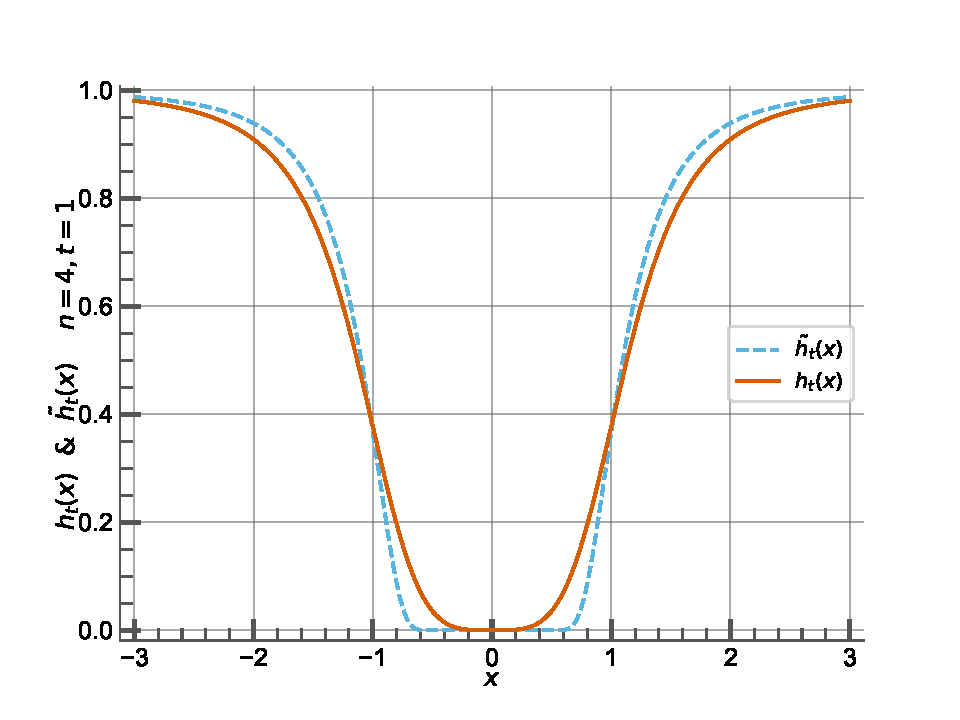
\includegraphics[width=0.49\linewidth]{chapter_1/assets/h_stable_vs_unstable.pdf}}
  \caption{\centering The unstable reparametrization function $h_t^*$ and its
  stable alternative $h_t$, with $t=1$ and $n=4$ for both functions.} 
  \label{fig:chap1:h_stable_vs_unstable}
\end{figure}

\subsection{Budget Loss}
\label{sec:chap1:budget_loss}

Most traditional pruning methods in deep learning do not explicitly incorporate
the target weight budget during the optimization procedure. The amount of
weights pruned is typically enforced post-training, which can lead to suboptimal
results compared to methods that consider the weight budget during optimization.
Our method introduces a budget loss term, in addition to the main task loss
term, that drives the network to match and respect a given weight budget during
the training process. Consequently, the trained network can be pruned to the
desired pruning rate with a marginal loss in accuracy and does not need
fine-tuning.\\


The considered budget is weight-based and should quantify the target fraction of
active connection in the network. To build the budget loss, we first introduce a
cost function that quantify the number of active connection in the network. Let
$C(\{\mathbf{w}_1,\dots, \mathbf{w}_L\})$ be the {\em current} cost associated
to a neural network and its set of {\em current} weights and $C_\text{target}$
the {\em targeted} one. $C_\text{target}$ is the number of connections that
should be active at the end of the training procedure. The budget loss is
defined as \\

\begin{equation}
  \label{eqn:chap1:simple_budget}
  {\cal L}_\text{budget} = \bigl( C(\{\mathbf{w}_1,\dots, \mathbf{w}_L\}) - C_\text{target} \bigr)^2.
\end{equation} \\


\noindent This budget loss is combined with the main task loss (that is a
classification loss in our experiments - see \cref{sec:chap1:experiments}). The
budget loss $ {\cal L}_\text{budget}$ is in quadratic form to ensure the
minimisation if this loss will in turn minimise the difference between the {\em
current} cost and the {\em targeted} one. For a better  conditioning of this
combination, we normalize the budget loss by $C_\text{initial}$. The latter
corresponds to the cost of the primary unpruned network and it is set in
practice to the number of its parameters (see also
\cref{sec:chap1:experiments}). Hence, \cref{eqn:chap1:simple_budget} is updated
as  \\

\begin{equation}
  \label{eqn:realbudget}
  {\cal L}_\text{budget} = \biggl( \displaystyle\frac{C(\{\mathbf{w}_1,\dots, \mathbf{w}_L\}) - C_\text{target}}{C_\text{initial}} \biggr)^2.
\end{equation}\\

Finally, the two losses are combined together via a strictly positive mixing
parameter $\lambda$ that  controls the relative importance of  the budget loss
${\cal L}_\text{budget}$ compared to the main task loss ${\cal L}_\text{task}$,
leading to\\

\begin{equation}
  \label{eqn:globalloss}
   {\cal L} =  {\cal L}_\text{task} + \lambda \cdot {\cal L}_\text{budget}.
\end{equation} \\

Ideally, the budget of a neural network could be evaluated as the number of
multiply-add operations, often referred as \ac{FLOPs}, needed for a forward pass
or through the $\ell_0$ norm of its weights. However, neither are known to be
differentiable and therefore cannot be used in a gradient-based optimization. In
order to circumvent this limitation, we use our weight reparametrizaion as a
surrogae measure of $\ell_0$ and we define the cost function as \\

\begin{equation}
  \label{eqn:chap1:cost_function}
  C(\{\mathbf{w}_1,\dots, \mathbf{w}_L\}) = \displaystyle \sum_{i=1}^{L} h_t(\mathbf{w}_i). 
\end{equation} \\


\begin{figure}
  \centering
  \subfloat[Number of parameters]{
      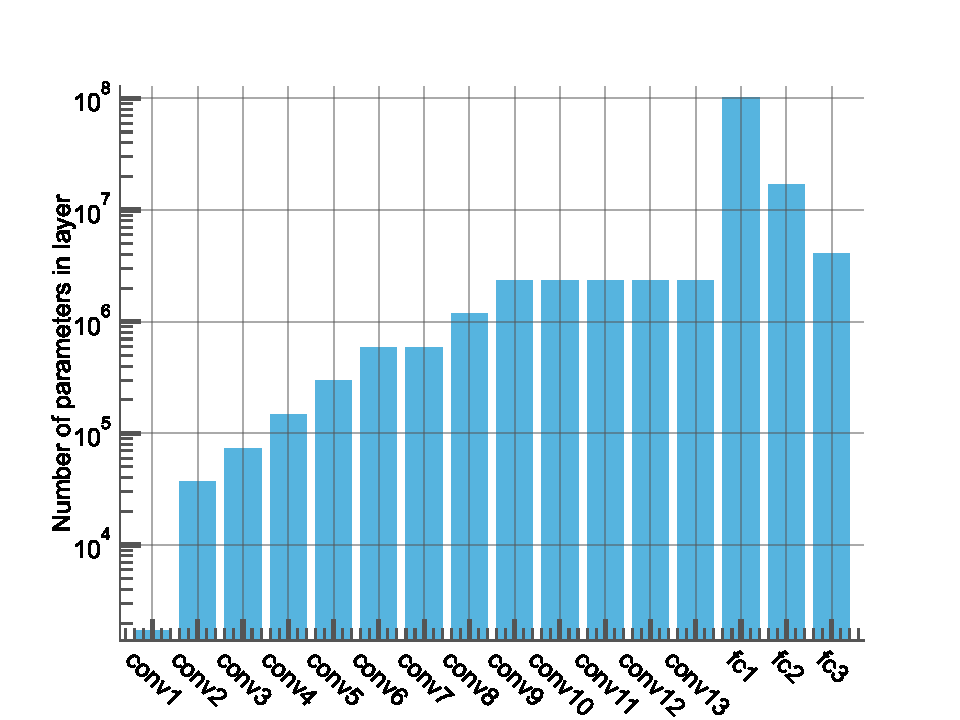
\includegraphics[width=0.49\linewidth]{chapter_1/assets/vgg16_num_params_per_layer.pdf}
      \label{fig:chap1:num_parap_vgg16}} \subfloat[Normalization factor]{
      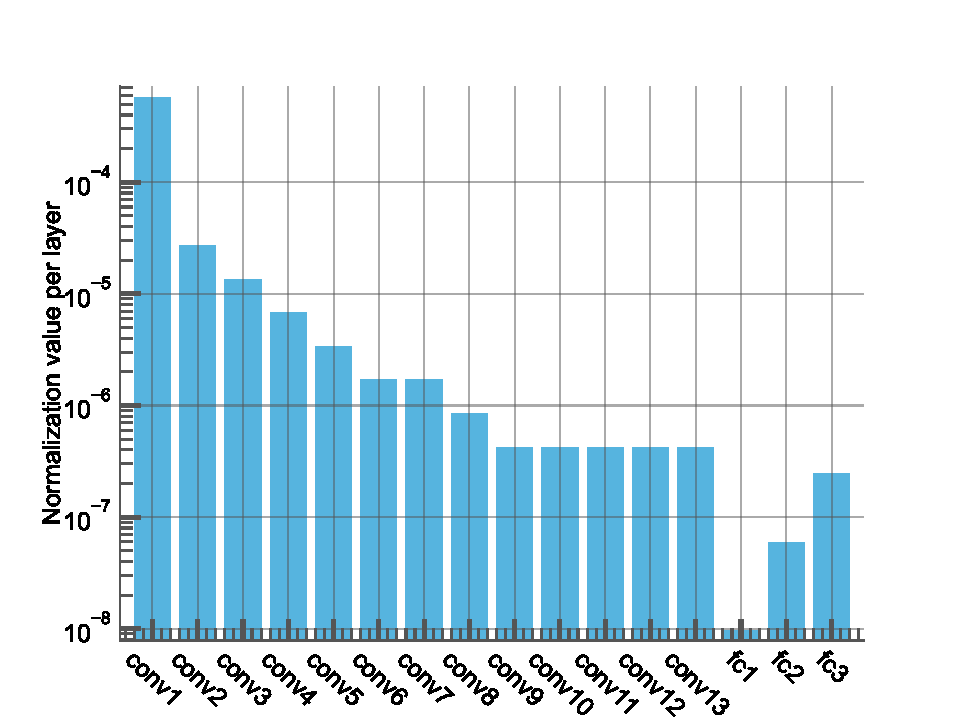
\includegraphics[width=0.49\linewidth]{chapter_1/assets/vgg16_normalization_factor_per_layer.pdf}
      \label{fig:chap1:norm_factor_vgg16}} \caption{\centering Log-scale plot of
      number of parameters and normalization factor per layer for a VGG16
      network. The significant differences in term of the number of parameters
      yields dramaticaly different normalization factors. Some of them are 4
      orders of magnitude appart, and all of them are vanishingly small compared
      to a standard main task loss value.} 
  \label{fig:chap1:vgg16_per_layer_param_and_norm_factor}
\end{figure}

One could argue that the cost should be normalized layer-wise and therefore that
the right hand term of \cref{eqn:chap1:cost_function} should be written as
$$\displaystyle\sum_{i=1}^{L}\frac{h_t(\mathbf{w}_i)}{\text{Card}(\mathbf{w}_i)}$$
where $\text{Card}(.)$ denotes the cardinal function, it is to say in this case
the number of scalar elements in a weight tensor. However, the number of
elements in a layer greatly varies from one layer to another (as demonstrated in
\cref{fig:chap1:vgg16_per_layer_param_and_norm_factor}). As a result,  the
budget loss relative importance would vary from one layer to another. More
importantly, the optimization process would have less incentive to introduce
sparsity in larger layers since their normalization factor would make the budget
loss negligable compared to other layers or the main task loss. This is critical
since the large layers are generaly the one where the highest pruning rates can
be achieved \cite{DBLP:journals/corr/abs-2202-12002}. Regarding the
aforementioned reasons, a better alternative is to normalize by the initial cost
$C_\text{initial}$, as done in \cref{eqn:realbudget}.\\

% endregion

\section{Experiments And Results}
\label{sec:chap1:experiments}

In this section, we will explore the effectiveness of our method on  deep neural
networks for image classification. We have chosen to use three reference
databases in the field of computer vision: CIFAR10 \cite{CIFARdataset}, CIFAR100
\cite{CIFARdataset}, and TinyImageNet \cite{TinyImageNet}. We will evaluate the
impact of our method on several neural network architectures: VGG16
\cite{DBLP:journals/corr/SimonyanZ14a}, Conv4 \cite{DBLP:conf/iclr/FrankleC19},
ResNet18, and ResNet20 \cite{DBLP:conf/cvpr/HeZRS16}. This study will allow us
to demonstrate the effectiveness of our method for compressing image
classification models, as well as its influence on prediction accuracy. To that
extent we will review the impact of both our reparametrization and our budget
loss.\\

The CIFAR10 and CIFAR100 datasets both contain 60,000 color images of size 32x32 pixels,
split in 10 and 100 classes respectively. The TinyImageNet dataset is shrunk version of
the ImageNet dataset \cite{DBLP:journals/ijcv/RussakovskyDSKS15}, and contains
100,000 images of size 64x64 pixels, split in 200 classes. Each dataset is
divided in to two folds: a training set and a test set. In addition to these two
folds, we also use a validation set to tune the hyperparameters of our method,
before testing it on the test set. The validation dataset is obtained by
selecting 10\% of the training set. \Cref{tab:chap1:datasets} summarizes the
composition of the three datasets.\\


\begin{table}[h]
  \centering
  \begin{tabular}{lcccc}
    \toprule
    \textbf{Dataset} & \textbf{Number of images} & \textbf{Number of classes} &
    \textbf{Image size} & \textbf{Size of test set} \\ 
    \hline
    CIFAR10 & 60,000 & 10 & 32x32 & 10,000 \\ 
    CIFAR100 & 60,000 & 100 & 32x32 & 10,000\\ 
    TinyImageNet & 100,000 & 200 & 64x64 &10,000 \\ 
    \bottomrule
  \end{tabular}
  \caption{The number of images, of classes, image size and size of the test set for the three datasets used.}
  \label{tab:chap1:datasets}
\end{table}

In combination with these datasets, we use four different neural networks. Conv4
is a small and reasonably lightweight convolutional neural network which is a
shrunk-down version of the VGG16 architecture. VGG16 is a convolutional neural
of larger size and depth, which is a popular choice for image classification, we
used a slightly modified version of VGG16 that is better suited to CIFAR10. We
do not use dropout but we use batch normalization, and the fully connected
section has only one layer. ResNet18 is a residual neural network that
introduces skip connection in its architectural design. ResNet20 is a modified
version of the ResNet18 architecture to make it suited for CIFAR10 and CIFAR100
datasets. \Cref{tab:chap1:networks_size} summarizes the size of the different
models. In our experiments, we use ResNet18 exclusively for TinyImageNet and the
other networks for CIFAR10 and CIFAR100.\\


\begin{table}[h]
  \centering
  \begin{tabular}{lllll}
  \cline{2-5}
                       & Conv4     & VGG16      & ResNet20 & ResNet18   \\ \hline
  Number of Parameters & 2,425,930 & 14,728,266 & 269,034  & 11,685,608 \\ \hline
  \end{tabular}
  \caption{\centering Number of parameters for the four neural network architectures used.}
  \label{tab:chap1:networks_size}
\end{table}

\subsection{Performances}
\label{sec:chap1:performances}
Performances of our method are evaluated on CIFAR10 and CIFAR100 with Conv4, VGG16
and ResNet20. On TinyImageNet, we evaluate our method on ResNet18. We compare
our method against magnitude pruning \cite{DBLP:conf/nips/HanPTD15}. The key
differences between our method and magnitude pruning are the following: $(i)$
our method uses a budget loss to encourage sparsity, which takes into account the
final pruning rate from the beginning of the training process, $(ii)$ our method
does not require fine-tuning after pruning. Because of the latter, we compare
our method against magnitude pruning with and without fine-tuning. Both methods
share the following setup: networks are trained during 300 epochs with an
initial learning rate of 0.1. A {\em Reduce On Plateau} policy is applied to the
learning rate: if the validation accuracy is not improving for 10 epochs in a
row, then the learning rate is decreased by a factor 0.3. A weight decay is
applied on the weights with a penalization factor of $5\times10^{−5}$. An Early
Stopping policy was used to stop prematurely the training if no improvement of
the test accuracy is observed in 60 epochs. To keep the comparison fair, for
magnitude pruning, the 300 epochs are split into two phases: the first 150 epochs
are dedicated to the training of the network, and the last 150 epochs are used
for fine-tuning the pruned network. In the fine-tuning phase, the learning rate
is divided by 100 to allow for better convergence. \\

Results are repported on
\cref{fig:chap1:reparam_vs_mpft_conv4,fig:chap1:reparam_vs_mpft_resnet20,fig:chap1:reparam_vs_mpft_vgg16}.
On the aforementioned figures, our method (denoted \emph{Ours}) is compared to
magnitude pruning with and without fine-tuning (denoted \emph{MP w/ FT} and
\emph{MP w/o FT}, respectively). All three methods are evaluated on the test
fold of the dataset once the network has been pruned up to the pruning rate
indicated on the \emph{x-axis}. The test accuracy is reported on the
\emph{y-axis} as a float between 0 and 1 (0 being all images wrongly classified
and 1 being all images correctly classified). Each solid line representing a
method is the mean of 5 independent runs. The colored area surrounding the solid
line represents the range within plus or minus one standard deviation. In
addition to the 3 methods, the dashed lines represent the performances of an
unpruned network trained without weight reparametrization and budget loss
(denoted \emph{baseline}) and the accuracy of our method before the effective
pruning (denoted \emph{Ours (pre pruning)}).\\

% region: perfs_figures
\begin{figure}
  \centering
  \subfloat[Conv4 - CIFAR10]{
      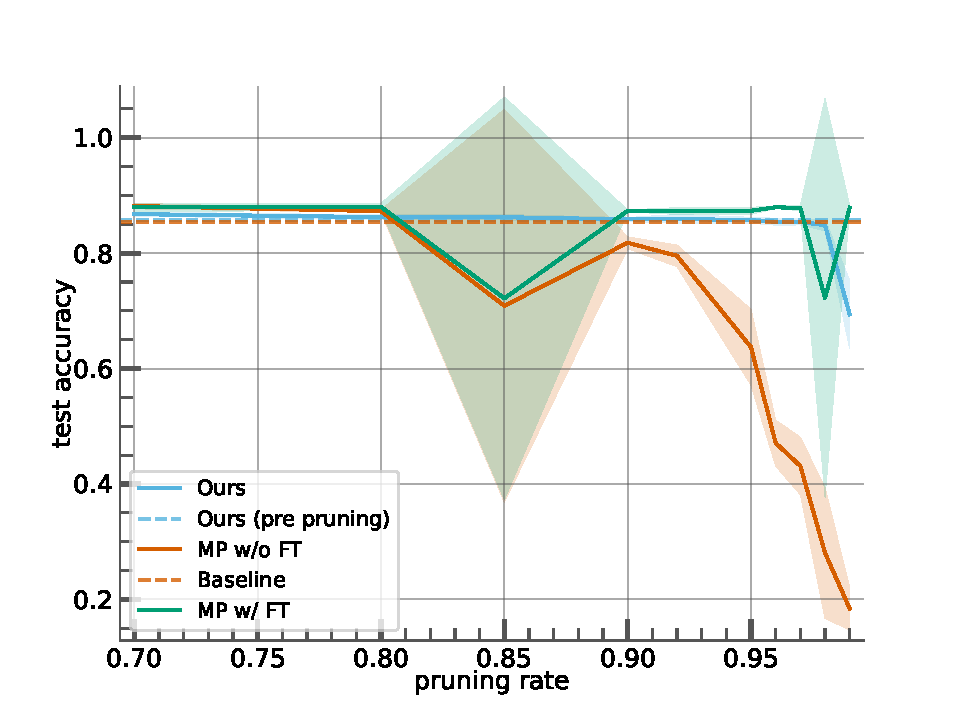
\includegraphics[width=0.49\linewidth]{chapter_1/assets/reparam_vs_mpft_Conv4_cifar10.pdf}
      \label{fig:chap1:reparam_vs_mpft_conv4_cifar10}}
  \subfloat[Conv4 - CIFAR100]{
      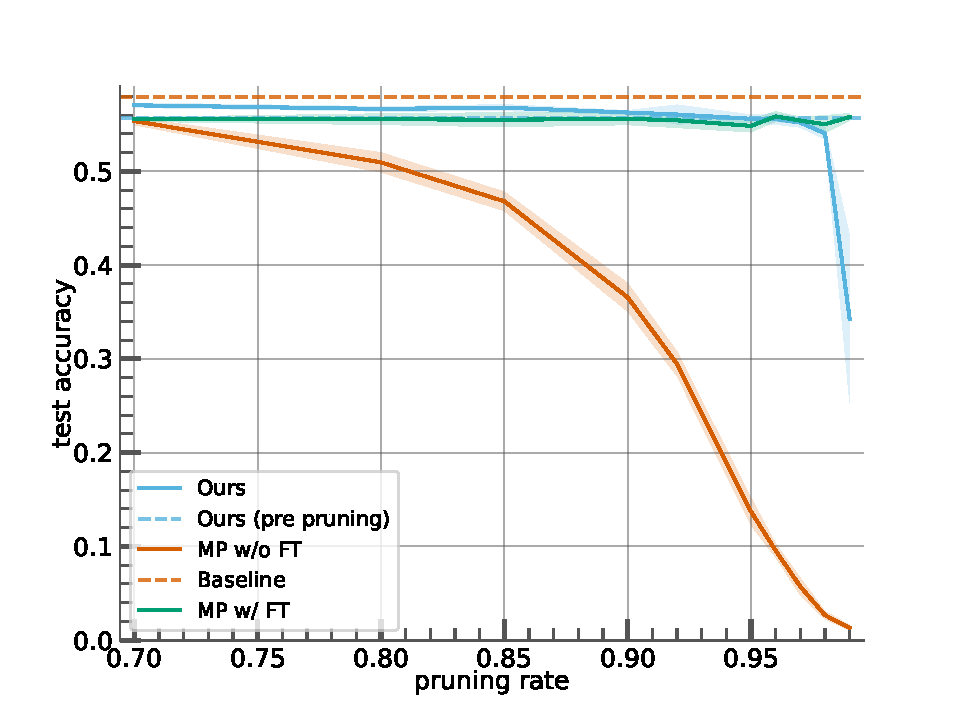
\includegraphics[width=0.49\linewidth]{chapter_1/assets/reparam_vs_mpft_Conv4_cifar100.pdf}
      \label{fig:chap1:reparam_vs_mpft_conv4_cifar100}}
      \\
  \subfloat[Conv4 - CIFAR10 (Number of Epochs)\label{fig:chap1:reparam_vs_mpft_conv4_cifar10_epochs}]{
      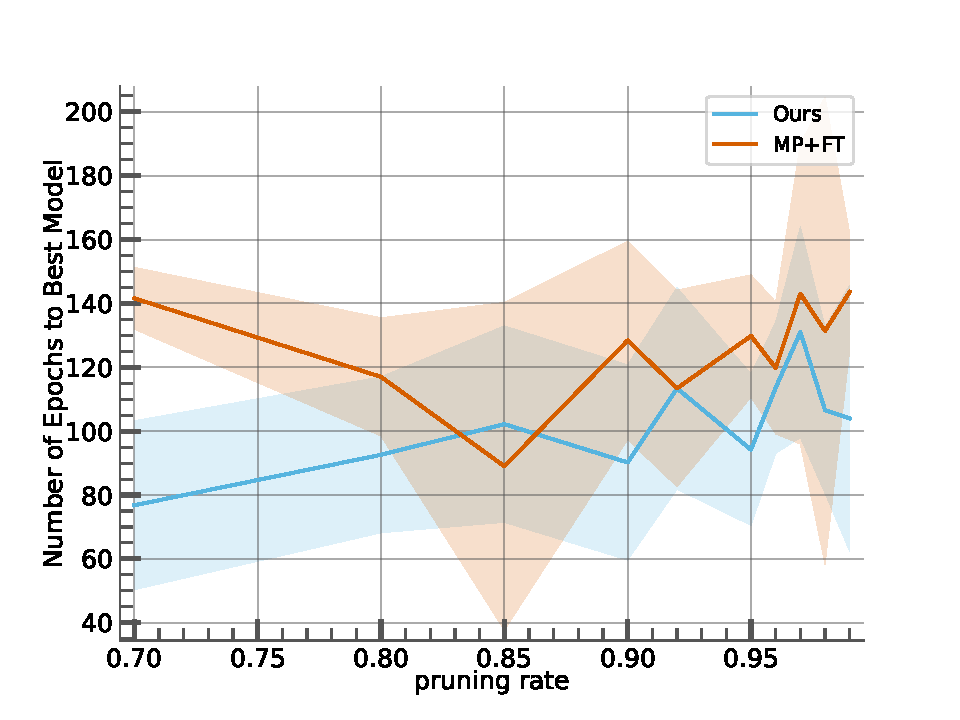
\includegraphics[width=0.49\linewidth]{chapter_1/assets/reparam_vs_mpft_training_time_Conv4_cifar10.pdf}}
  \subfloat[Conv4 - CIFAR100 (Number of Epochs)\label{fig:chap1:reparam_vs_mpft_conv4_cifar100_epochs}]{
      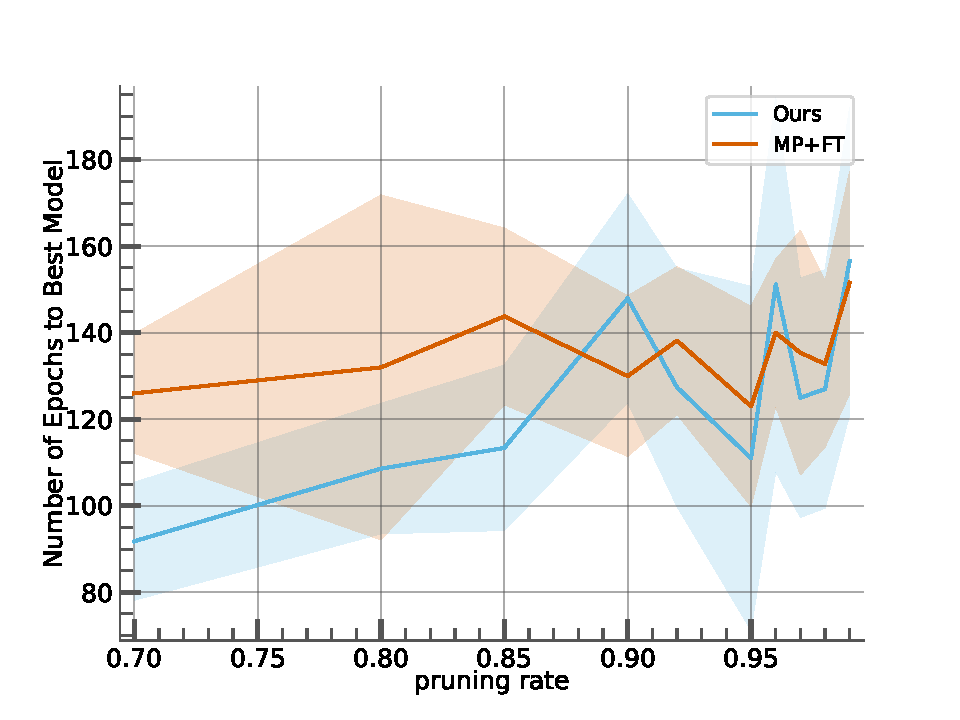
\includegraphics[width=0.49\linewidth]{chapter_1/assets/reparam_vs_mpft_training_time_Conv4_cifar100.pdf}}
  \caption{\centering Performances comparison of our method {\em(Ours)} against
  magnitude pruning without {\em(MP w/o FT)} and with fine-tuning {\em(MP w/ FT)} with a Conv4 network on
  CIFAR10 and CIFAR100 datasets, for different pruning rates.
  \Cref{fig:chap1:reparam_vs_mpft_conv4_cifar10} and
  \cref{fig:chap1:reparam_vs_mpft_conv4_cifar100} show the testing accuracy of
  the model and \cref{fig:chap1:reparam_vs_mpft_conv4_cifar10_epochs} and
  \cref{fig:chap1:reparam_vs_mpft_conv4_cifar100_epochs} the number of epochs
  needed to obtain the best model.}
  \label{fig:chap1:reparam_vs_mpft_conv4}
\end{figure}

\begin{figure}
  \centering
  \subfloat[VGG16 - CIFAR10]{
      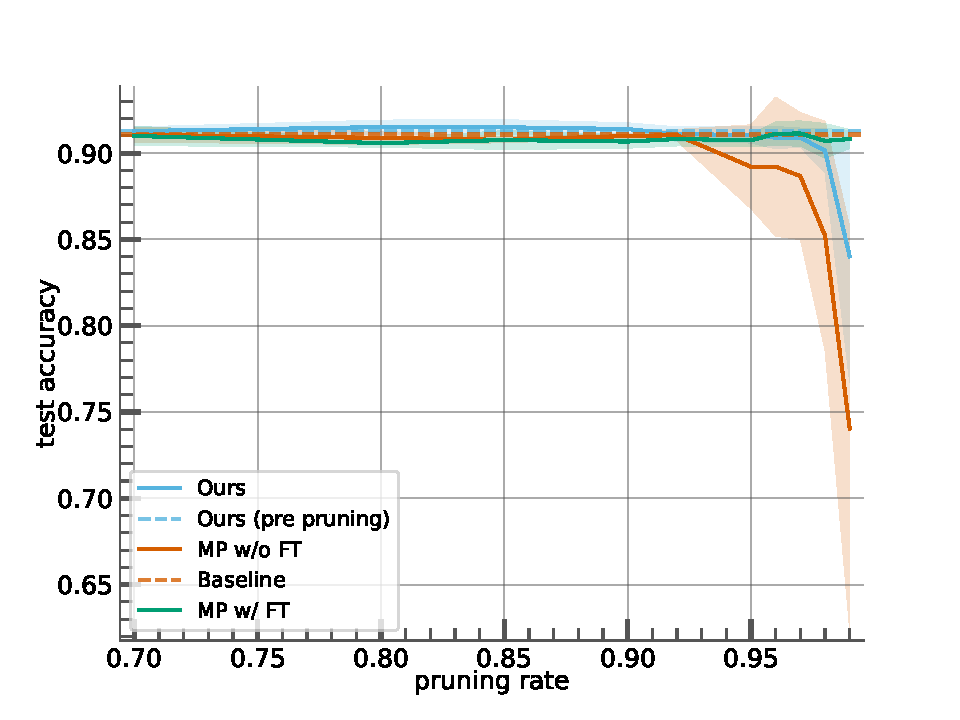
\includegraphics[width=0.49\linewidth]{chapter_1/assets/reparam_vs_mpft_PrunableVGG16_cifar10.pdf}
      \label{fig:chap1:reparam_vs_mpft_vgg16_cifar10}} 
  \subfloat[VGG16 - CIFAR100]{
      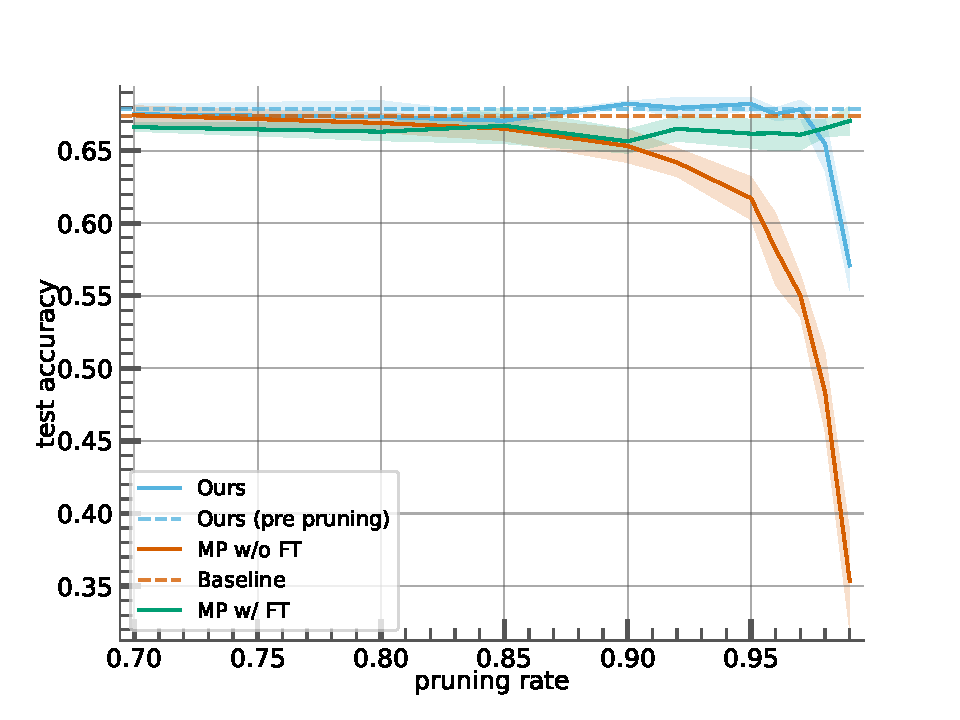
\includegraphics[width=0.49\linewidth]{chapter_1/assets/reparam_vs_mpft_PrunableVGG16_cifar100.pdf}
      \label{fig:chap1:reparam_vs_mpft_vgg16_cifar100}} 
  \\
  \subfloat[VGG16 - CIFAR10 (Number of Epochs)\label{fig:chap1:reparam_vs_mpft_vgg16_cifar10_epochs}]{
    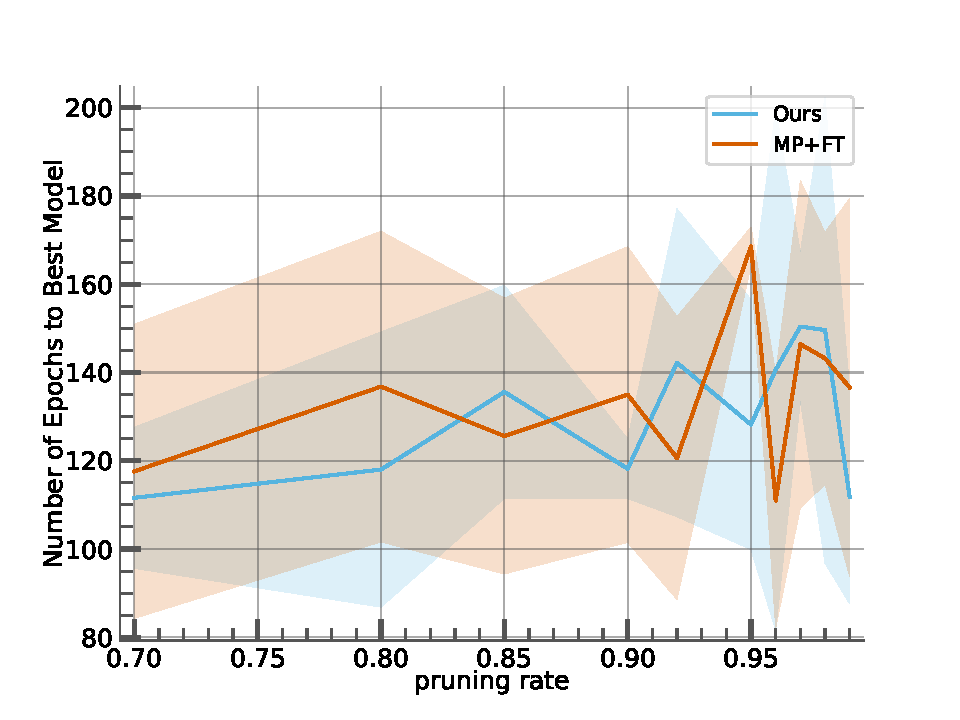
\includegraphics[width=0.49\linewidth]{chapter_1/assets/reparam_vs_mpft_training_time_PrunableVGG16_cifar10.pdf}}
  \subfloat[VGG16 - CIFAR100 (Number of Epochs)\label{fig:chap1:reparam_vs_mpft_vgg16_cifar100_epochs}]{
      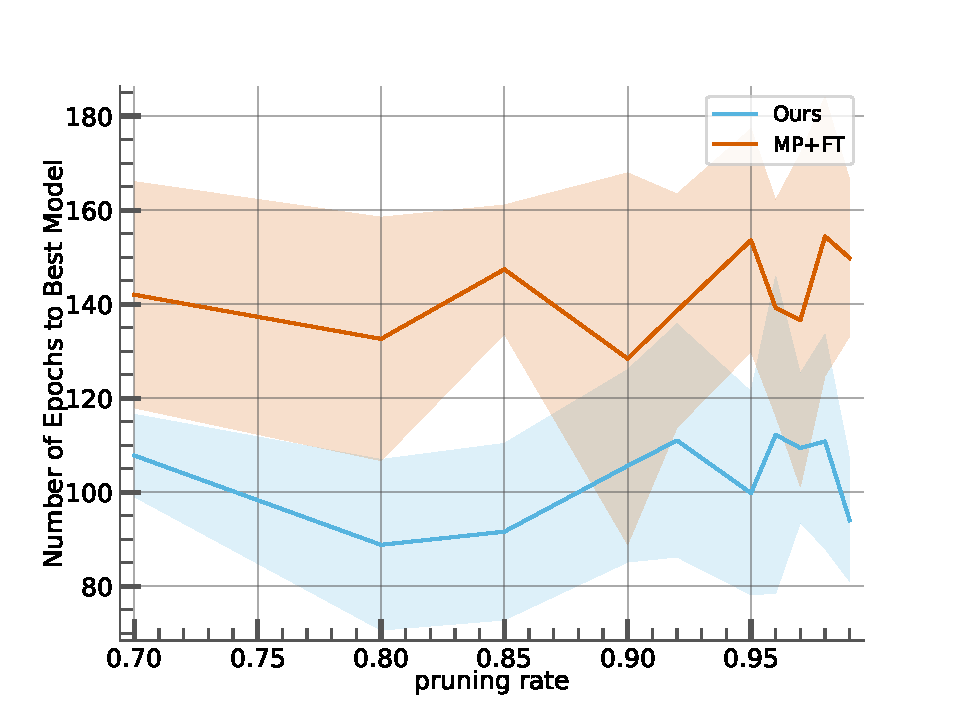
\includegraphics[width=0.49\linewidth]{chapter_1/assets/reparam_vs_mpft_training_time_PrunableVGG16_cifar100.pdf}}

    
  \caption{\centering Performances comparison of our method \em{(Ours)} against
  magnitude pruning with fine-tuning \em{(MP+FT)} with a VGG16 network on
  CIFAR10 and CIFAR100 datasets, for different pruning rates.
  \Cref{fig:chap1:reparam_vs_mpft_vgg16_cifar10} and
  \cref{fig:chap1:reparam_vs_mpft_vgg16_cifar100} show the testing accuracy of
  the model and \cref{fig:chap1:reparam_vs_mpft_vgg16_cifar10_epochs} and
  \cref{fig:chap1:reparam_vs_mpft_vgg16_cifar100_epochs} the
  number of epochs needed to obtain the best model.}
  \label{fig:chap1:reparam_vs_mpft_vgg16}
\end{figure}

\begin{figure}
  \centering
  \subfloat[ResNet20 - CIFAR10\label{fig:chap1:reparam_vs_mpft_resnet20_cifar10}]{
      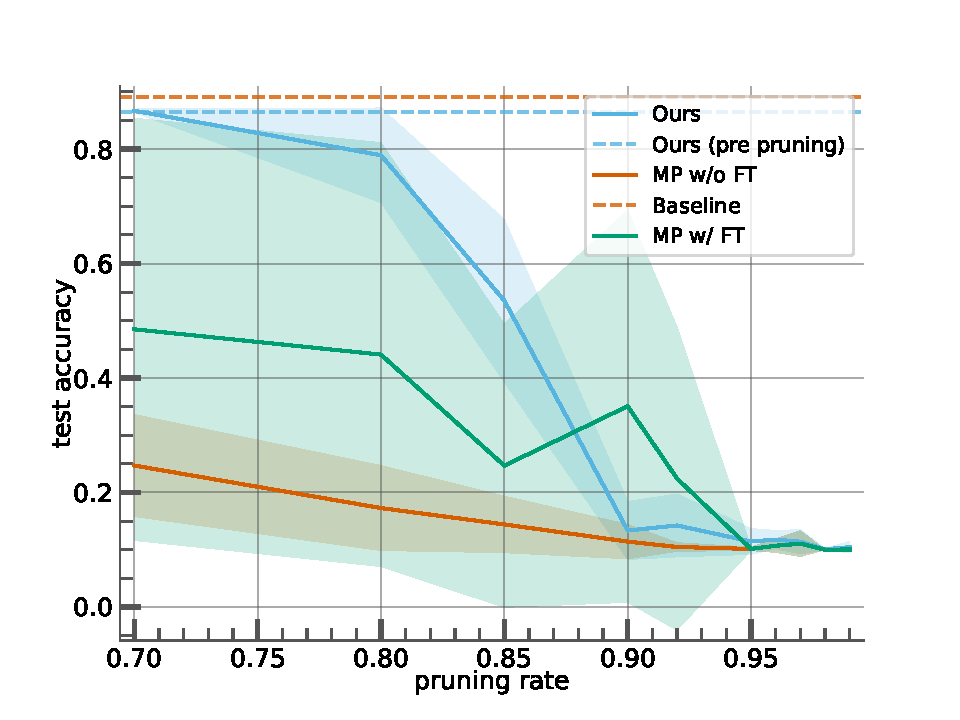
\includegraphics[width=0.49\linewidth]{chapter_1/assets/reparam_vs_mpft_PrunableResNet20_cifar10.pdf}}
  \subfloat[ResNet20 - CIFAR100\label{fig:chap1:reparam_vs_mpft_resnet20_cifar100}]{
      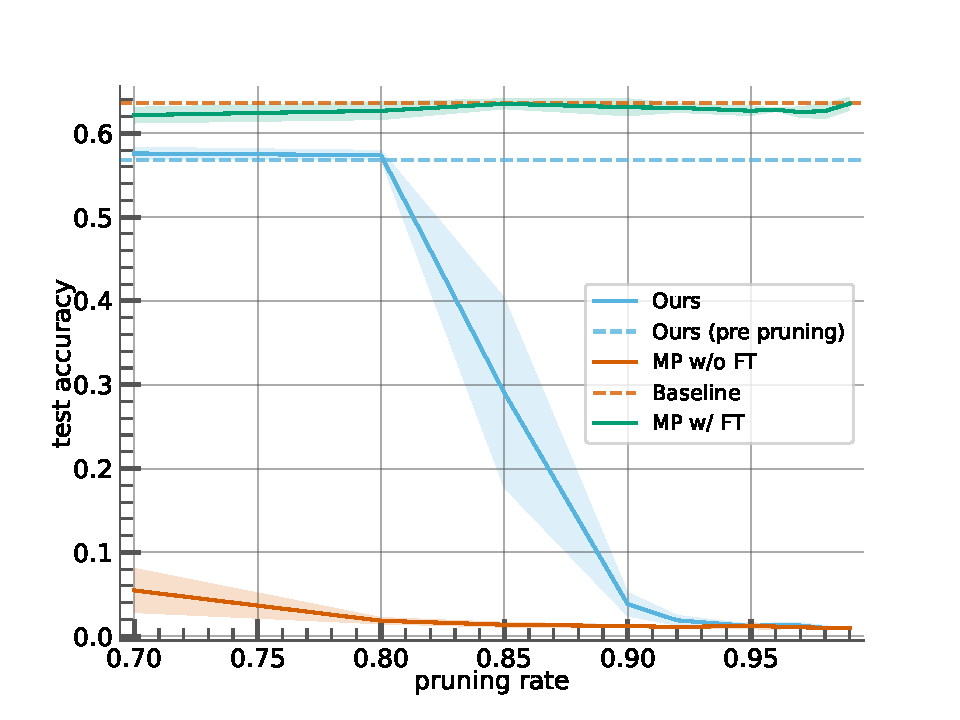
\includegraphics[width=0.49\linewidth]{chapter_1/assets/reparam_vs_mpft_PrunableResNet20_cifar100.pdf}} 
  \\
  \subfloat[ResNet20 - CIFAR10 (Number of Epochs)\label{fig:chap1:reparam_vs_mpft_resnet20_cifar10_epochs}  ]{
      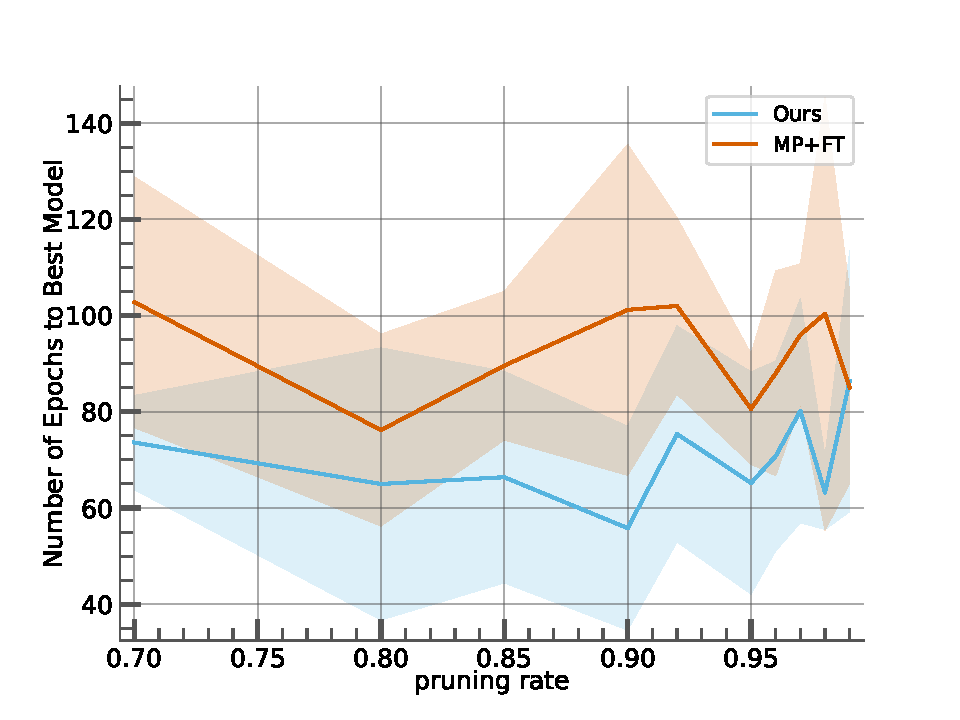
\includegraphics[width=0.49\linewidth]{chapter_1/assets/reparam_vs_mpft_training_time_PrunableResNet20_cifar10.pdf}}
  \subfloat[ResNet20 - CIFAR100 (Number of Epochs)\label{fig:chap1:reparam_vs_mpft_resnet20_cifar100_epochs}]{
      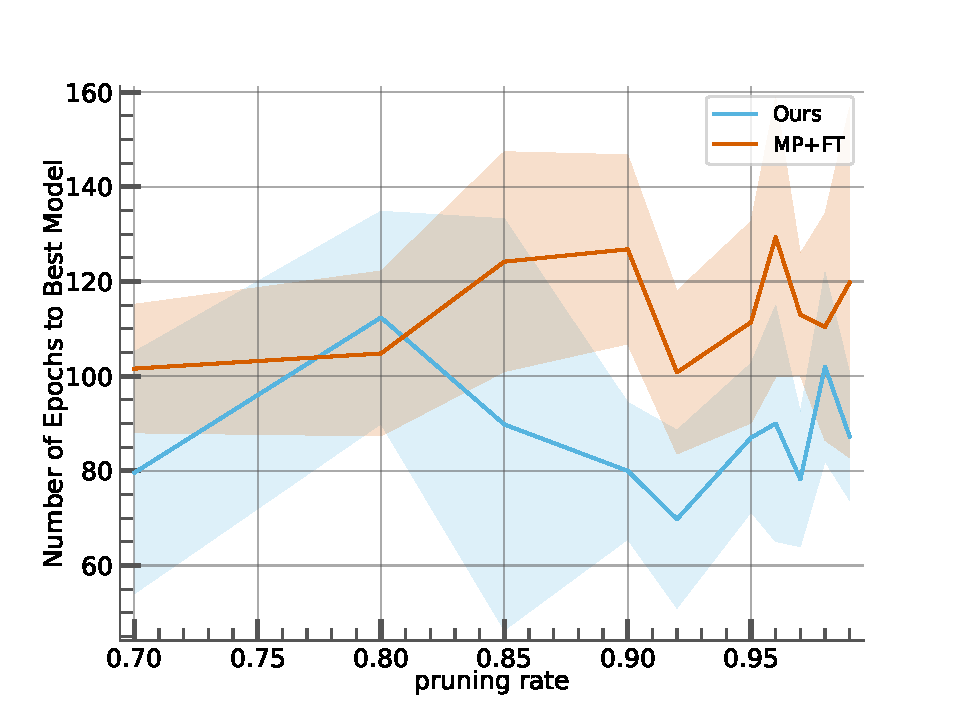
\includegraphics[width=0.49\linewidth]{chapter_1/assets/reparam_vs_mpft_training_time_PrunableResNet20_cifar100.pdf}}
  \caption{\centering Performances comparison of our method \em{(Ours)} against
  magnitude pruning with fine-tuning \em{(MP+FT)} with a ResNet20 network on
  CIFAR10 and CIFAR100 datasets, for different pruning rates.
  \Cref{fig:chap1:reparam_vs_mpft_resnet20_cifar10} and
  \cref{fig:chap1:reparam_vs_mpft_resnet20_cifar100} show the
  testing accuracy of the model and
  \cref{fig:chap1:reparam_vs_mpft_resnet20_cifar10_epochs} and
  \cref{fig:chap1:reparam_vs_mpft_resnet20_cifar100_epochs}
  the number of epochs needed to obtain the best model.}
  \label{fig:chap1:reparam_vs_mpft_resnet20}
\end{figure}

% endregion: perfs_figures

\subsection{Impact of \texorpdfstring{$\lambda$}{Lambda}}
\label{sec:chap1:impact_of_lambda}

See \cref{fig:chap1:lambda_impact} for the impact of $\lambda$ on the respect
of the budget. Low pruning rate on \cref{fig:chap1:lambda_impact_pruning_90} and
high pruing rates on \cref{fig:chap1:lambda_impact_pruning_95} are obtained.
The tradeoff between the budget loss and the main task loss is clearly visible
on table \ref{tab:chap1:lambda_impact}. 

\begin{table}[tbp]
  \centering
  \begin{center}
    \begin{tabular}{llcc}
      \toprule
      Pruning Rate & $\lambda$ & Achieved Budget & Test Accuracy (post pruning) \\
      \midrule
      \multirow{4}{*}{0.9} & 0.005 & 5.25 $\pm$ 0.69 & 85.83 $\pm$ 0.83 \\
      & 0.5 & 8.06 $\pm$ 0.19 & 86.34 $\pm$ 0.64 \\
      & 5 & 9.93 $\pm$ 0.03 & 85.82 $\pm$ 0.74 \\
      & 50 & \textbf{10.00 $\pm$ 0.01} & \textbf{86.52 $\pm$ 0.46} \\
      \midrule
      \multirow{4}{*}{0.95} & 0.005 & 5.22 $\pm$ 0.73 & \textbf{86.27 $\pm$ 0.32} \\
      & 0.5 & 4.33 $\pm$ 0.41 & 85.66 $\pm$ 0.74 \\
      & 5 & 4.85 $\pm$ 0.19 & 86.11 $\pm$ 0.48 \\
      & 50 & \textbf{5.03 $\pm$ 0.02} & 85.37 $\pm$ 0.37 \\
      \midrule
      \multirow{4}{*}{0.99} & 0.005 & 4.60 $\pm$ 0.29 & 40.52 $\pm$ 5.27 \\
      & 0.5 & 3.69 $\pm$ 0.38 & 42.45 $\pm$ 9.02 \\
      & 5 & 1.89 $\pm$ 0.45 & \textbf{76.85 $\pm$ 6.34} \\
      & 50 & \textbf{2.09 $\pm$ 0.15} & 10.00 $\pm$ 0.00 \\
      \bottomrule
    \end{tabular}
  \end{center}
  \caption{\centering
    Impact of the parameter $\lambda$ on the achieved budget and the post-pruning test accuracy of the model for a Conv4 network on CIFAR10 dataset,
    for various pruning rates. Although a high value of $\lambda$ ensures that
    the target budget is reached, it also leads to a lower test accuracy when
    the pruning rate increases.}
    \label{tab:chap1:lambda_impact}
\end{table}



\subsection{Impact of the budget loss}
\label{sec:chap1:impact_of_budget_loss}

% \subsection{Impact of the reparametrization}
% \label{sec:chap1:impact_of_reparametrization}

\subsection{Fine tuning context}
\label{sec:chap1:impact_of_fine_tuning}



\begin{figure}
\centering
\subfloat[Pruning 90\% of the weights\label{fig:chap1:lambda_impact_pruning_90}]{
  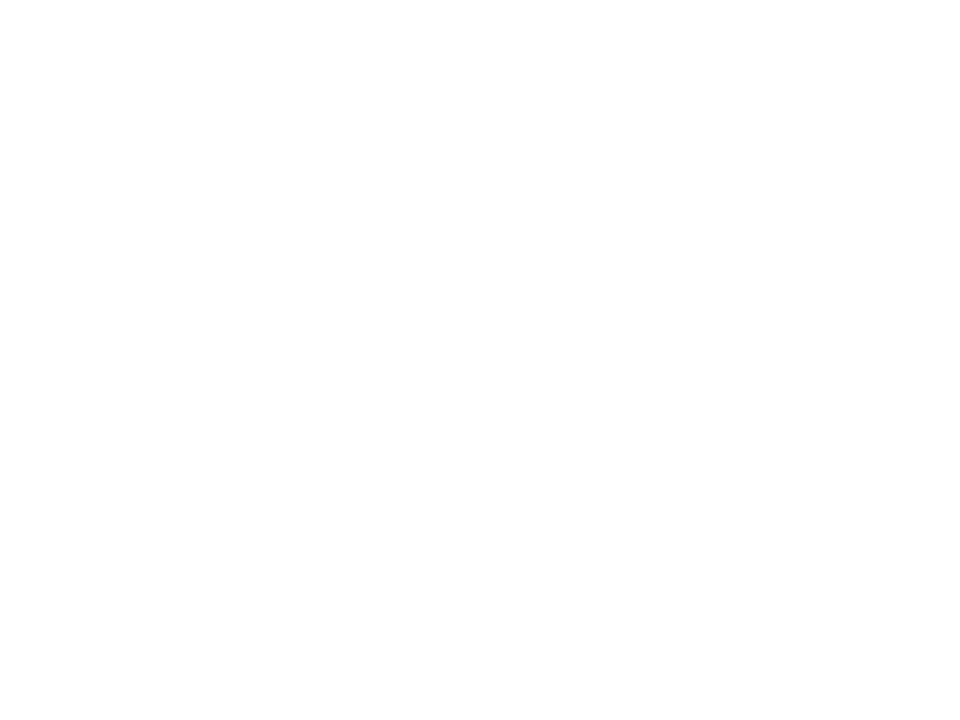
\includegraphics[width=0.49\linewidth]{chapter_1/assets/lambda_impact_pr_90_C4_CIFAR10.pdf}}
\subfloat[Pruning 95\% of the weights\label{fig:chap1:lambda_impact_pruning_95}]{
  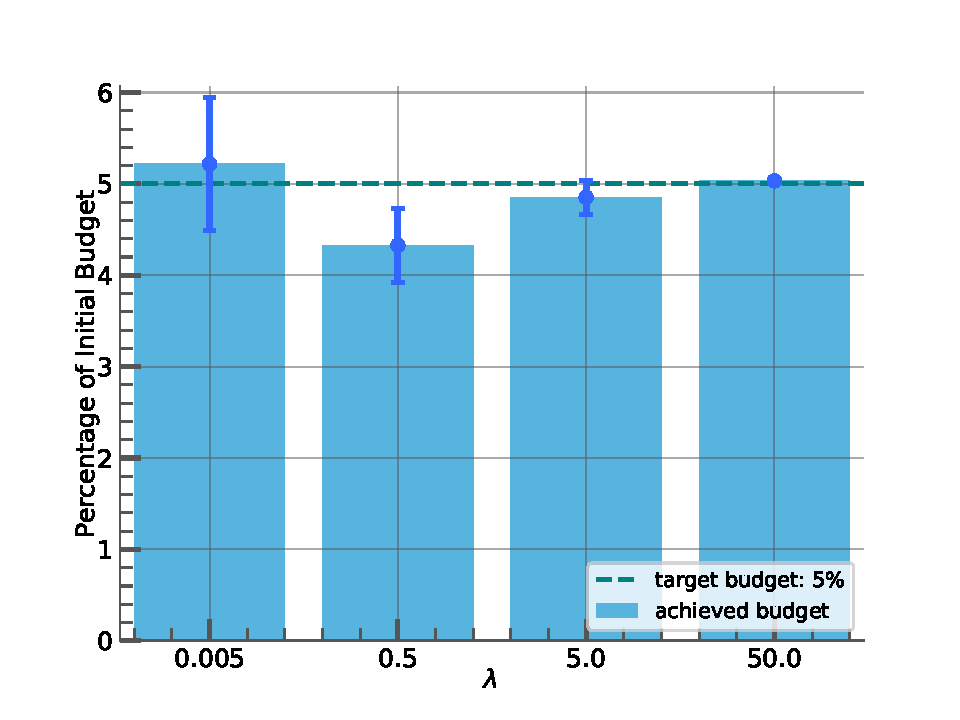
\includegraphics[width=0.49\linewidth]{chapter_1/assets/lambda_impact_pr_95_C4_CIFAR10.pdf}}
\\
\subfloat[Pruning 99\% of the weights\label{fig:chap1:lambda_impact_pruning_99}]{
  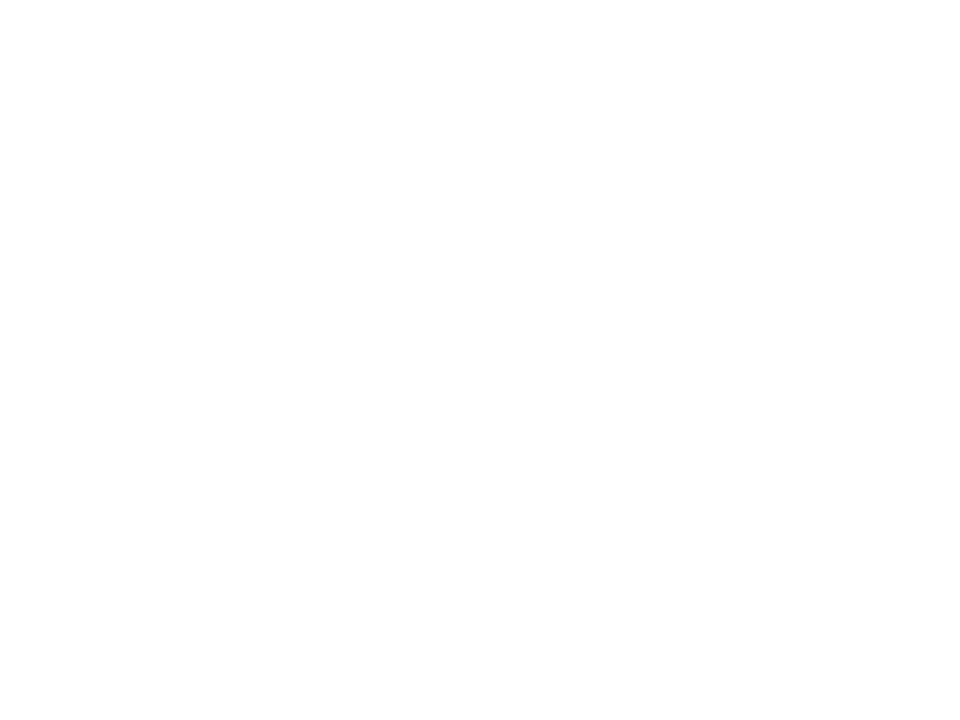
\includegraphics[width=0.49\linewidth]{chapter_1/assets/lambda_impact_pr_99_C4_CIFAR10.pdf}}
  \caption{\centering Impact of the parameter $\lambda$ on the achieved final
  budget for a Conv4 network on CIFAR10 dataset, for various pruning rates. A
  too-small value of $\lambda$ does not make the actual budget match the desired
  budget. The actual budget is either too small
  (\cref{fig:chap1:lambda_impact_pruning_90}) or too high
  (\cref{fig:chap1:lambda_impact_pruning_99}) compared to the target, depending
  on the applied pruning rate.}
\label{fig:chap1:lambda_impact}
\end{figure}  

